\section{Methodology}
\label{s:methodology}
As mentioned in ~\autoref{s:related-work}, there are two challenges in cloaking
detection: reveal the content and handle dynamics of a webpage.

In order to model the dynamics of a webpage, we propose Simhash-based Website
Model, that is, use clusters learned from fuzzy hashs to model average and
variance of each change. This is based on the assumption that, the content and
layout of a website delivered to different users each time, is consistent
despite of the dynamic part on the page, e.g. advertisements. In order to reveal
the uncloaked content, we design and implement simhash algorithm as browser
plugin, enabling crowdsourcing from user side.
Besides, we demonstrate the complexity of simhash algorithm, and show
that this plugin introduces negligible overhead to user browser.

\subsection{Simhash-based Website Model}
\subsubsection{Distance Approximation}
Simhash~\cite{charikar2002similarity} is a dimensionality reduction technique.
It is a fuzzy hash function family that maps a high dimension dataset into fixed
bits and preserves the following properties: 
(A) The fingerprint of a dataset is a “hash” of its features, and (B) The
hamming distance between two hash values is an estimation of the distance
between the original datasets.
This is different from 
cryptographic hash functions like SHA-1 or MD5, because they will hash two
documents which differs by single byte into two completely different hash-values and the
hamming distance between them is meaningless. 
However, simhash will hash them into similar hash-values.

In modeling the content and layout change of a website, we want to do learning
and comparing on a per url basis, therefore, we are assuming that the small hamming
distance between 

Since we are modeling website on a per url basis and parameters in url may
change every time of visit, it is necessary to define the granurity of
comparison. We took a simplified approach, we simply strip all the parameter
values and keep all the parameter names, and throw away the scheme field, i.e.
{\it http://www.gatech.edu/?user=1234} is simplified to
{\it //www.gatech.edu/?user=}


%However, simhash
%will hash them into similar hash-values (the Hamming distance would be small).
%In designing a near-duplicate detection system based on simhash, one has to deal
%with the quaintness of simhash de- scribed above. The strategy we employed is as
%follows: we design our algorithms assuming that Property A holds, i.e., the
%fingerprints are distributed uniformly at random, and we experimentally measure
%the impact of non-uniformity intro- duced by Property B on real datasets.


%Suppose P and Q are probability distributions over L, 
%\begin{multline}
%  EMD(P, Q) \le E[d(h(P), h(Q))] \\
%  \le O(\log{n}\log{\log{n}})EMD(P, Q).
%\end{multline}
%
%This equation is telling us that the hamming distance between simhash of set
%\b{P} and set \b{Q} is an approximation of Earth Moving Distance(EMD) between set P
%and Q. Charikar~\cite{charikar2002similarity} give the formal proof that the
%hamming distance of sets represents the cosine similarity.
%~\cite{manku2007detecting} implements an algorithm for creating text-based
%simhash for a website. In our work, we use the same simhash algorithm,

\subsubsection{Computation}
In terms of simhash computation, we use the same settings described in 
~\cite{manku2007detecting}, which turns out to be effective given the corpus of
5 billion websites over the Internet.

The computation of simhash start from a set of features.
Given a set of features extracted from a document and their corresponding
weights, we use simhash to generate an f-bit fingerprint as follows. We maintain
an f-dimensional vector V, each of whose dimensions is initialized to zero.
A feature is hashed into an f-bit hash value. These f bits (unique to the
feature) increment/decrement the f components of the vector by the weight of
that feature as follows: if the i-th bit of the hash value is 1, the i-th com-
ponent of V is incremented by the weight of that feature; if the i-th bit of the
hash value is 0, the i-th component of V is decremented by the weight of that
feature. When all features have been processed, some components of V are
positive while others are negative. The signs of components determine the
corresponding bits of the final fingerprint.
In this work, f is set to 64.

\subsubsection{Insights On Feature Set Selection}
From the computation of the simhash, we can draw two insights:
(A) The order of the features in the original dataset does not matter, because
the algorithm randomly projects each feature to f-dimensional vector and count
the weighted presence in each dimension.
(B) Size of the feature set should be relatively large. Simhash is known to
perform badly on near duplicate detection when there are feature words. The
reason is that, when the number of features are small, each feature votes too
much on the vectors, difference in one feature may result in many bits of
difference.

Insight (A) is telling us, if the order of the original feature matters, the feature
set should cover this. Insight (B) means, simhash works on relatively large
number of datasets. The two insights are used in designing the text and dom
simhash.

\subsubsection{Text Simhash and Dom Simhash}


%
%Charikar’s simhash [17] is a dimensionality reduction tech- nique. It maps
%high-dimensional vectors to small-sized fin- gerprints. It is applied to
%web-pages as follows: we first con- vert a web-page into a set of features, each
%feature tagged with its weight. Features are computed using standard IR
%techniques like tokenization, case folding, stop-word removal, stemming and
%phrase detection. A set of weighted features constitutes a high-dimensional
%vector, with one dimension per unique feature in all documents taken together.
%With simhash, we can transform such a high-dimensional vector into an f-bit
%fingerprint where f is small, say 64.
%
%
%In order to compress text information of a document, we extract the same set of
%text features as ~\cite{manku2007detecting}.
%
%Inspired from previous work, we understand that looking at only text would raise
%high false positive, therefore, we take into consideration the tag.
%
%In order to compress the structural 
%
%for compressing
%the text information. 
%


In order to detect cloaking, we need to capture the bahavior and similarity that
a same website maintains. That is to say, we not only need to look at the text-based simhash,
but also dom-based simhash. We implemented the text-simhash algorithm 
same as the simhash algorithm used in spam detection by Google.
%described
%in ~\cite{manku2007detecting},
This algorithm extract words, bi-gram, tri-gram set
(repeated elements only recorded once) from a website and compute simhash using
simhash algorithm described in ~\cite{charikar2002similarity}. 
Because there are usually large number of words on a website, insight (B)
suffices. Besides, bi-gram, tri-gram is essentially the structure of the document,
thus insight (A) suffices.
This approach
and has great benefit in our use scenario, because this requires a single pass
of the document and no extra information. In contrast,
~\cite{manku2007detecting} implement extract weighted features using standard IR
techniques like tokenization, case folding, stop-word removal, stemming and
phrase detection, and may introduce more overhead and need extra knowledge.

\begin{figure}[t]
  \centering
  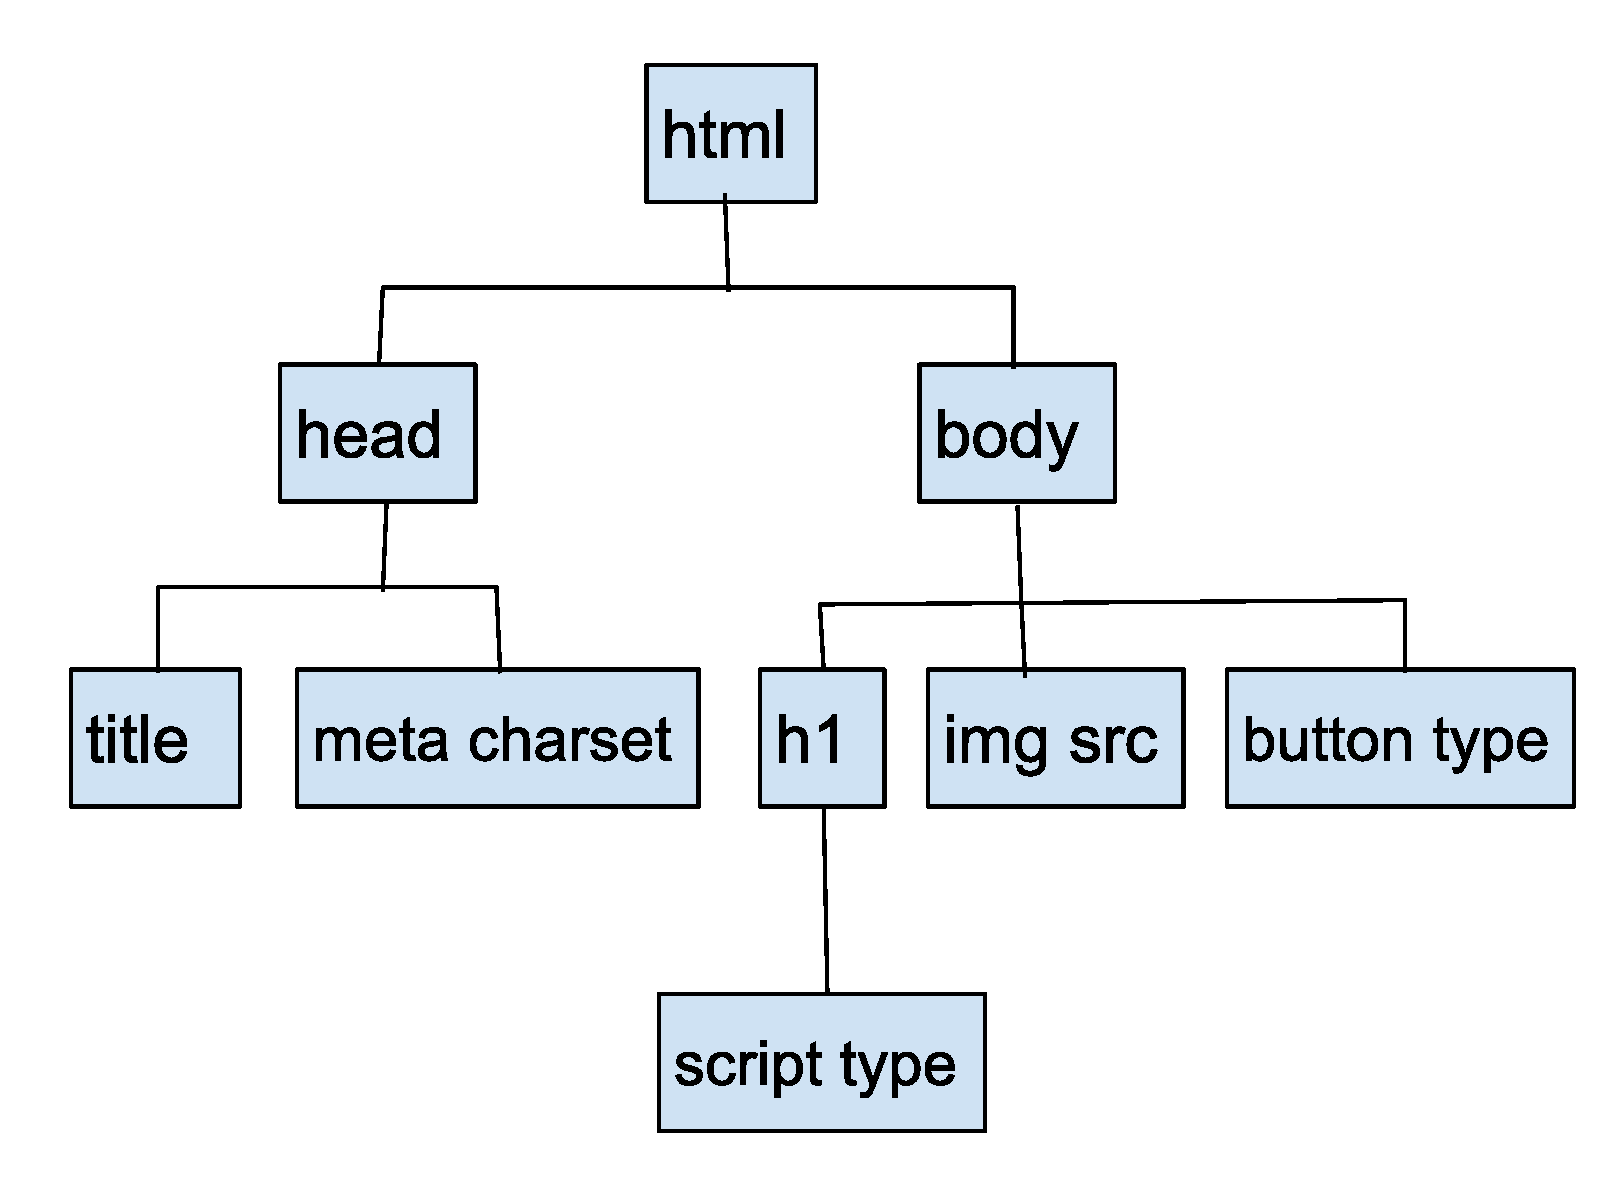
\includegraphics[width=.5\textwidth]{fig/dom-tree}
  \caption{DOM tree example}
  \label{fig:dom-tree}
\end{figure}

The content of a web page, Document Object Model (DOM), is organized in the form of a tree.
Figure ~\autoref{fig:dom-tree} shows a typical dom tree.
There is no current algorithm for generating dom simhash. Therefore, we design
an algorithm based on drawn insights.

For each dom tree, we record presence of each node, as
well as presence of each child parent pair. The node set tells us information about what
tag is present in this page, and child parent pair tells us how these tags are
organized, suffices insight (B). And the number of features extracted in this
fashion is relatively large, suffices insight (A).

% you can also use the wonderful epsfig package...
\begin{figure}[t]
  \centering
  \begin{subfigure}
    \centering
    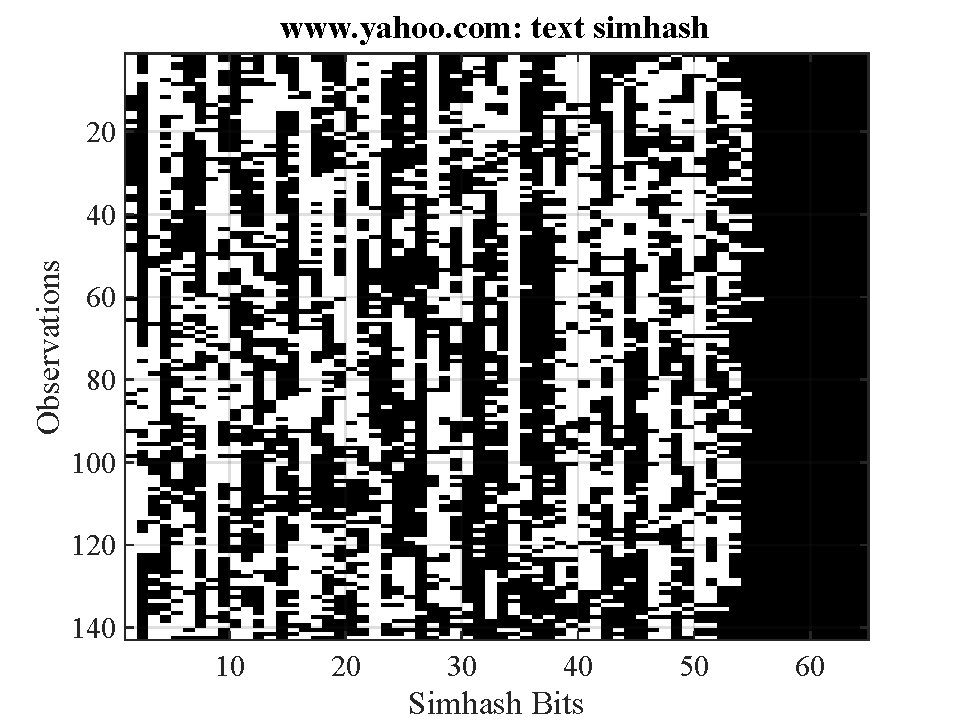
\includegraphics[width=.5\textwidth]{fig/yahoo-text-user}
    \label{fig:yahoo-text-user}
  \end{subfigure}%
  \begin{subfigure}
    \centering
    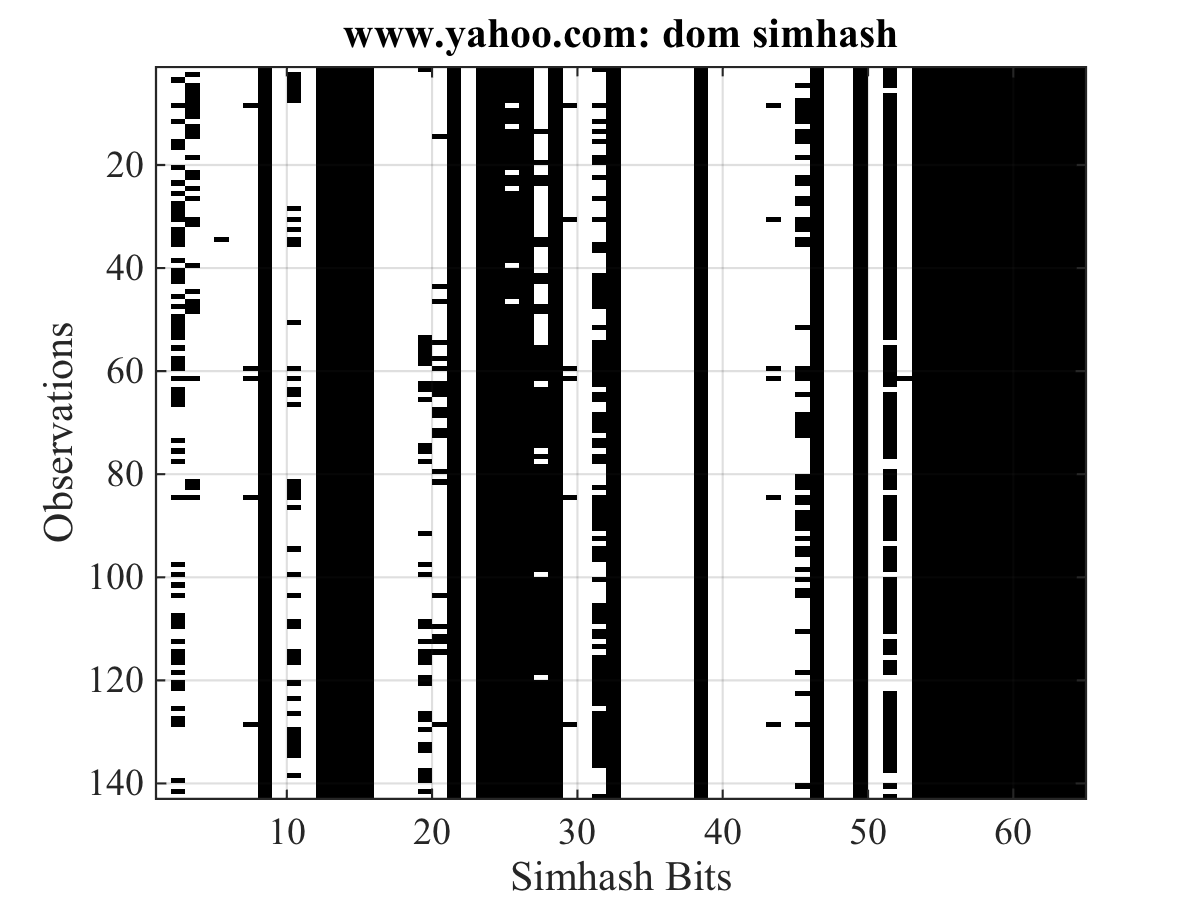
\includegraphics[width=.5\textwidth]{fig/yahoo-dom-user}
    \label{fig:yahoo-dom-user}
  \end{subfigure}
  \caption{Yahoo simhash changes over 7x24 period Feb.1 - 7, 2015}
  \label{fig:yahoo-simhash}
\end{figure}

It is pretty straightforward from ~\autoref{fig:yahoo-simhash} that,
text simhash changes rapidly, indicating dynamic nature of this
website, and dom simhash changes relatively slow and less.

Till now, we have demonstrated the algorithm we are using to generate
text-simhash and dom-simhash out of a website. Based on our observation, the
text-simhash may change rapidly, while dom-simhash relatively remain the same.

\subsubsection{Aggregating / Clustering}
Assume we are monitoring the same website over a period of time. This website
have dynamic changes all the time. But there can be another kind of change -
whole page change. In this case, it is reasonable to first separate them apart
and look at each of them.

Different from ~\cite{manku2007detecting}, we not only want to know whether two pages are
duplicate, we also want to know the patterns of these simhash. In this work, we employ
hierarchical clustering to do this job.

Since simhash maps a hight dimensional
features set into fixed number of bits, where hamming distance represents the
similarity between the original feature set. We leverage the fact that hamming
distance is euclidean distance (L1 norm on 64 dimension). On each dimension, the
original value is either 0 or 1. But it can be averaged and centriod can be
computed.

In this work, we use hierarchical clustering ~\cite{jones2014scipy} to cluster
collected simhash. The distance metric used is hamming distance, the linkage
method used is average. Criterion used is inconsistent coefficient.

These choice is actually straightforward. {\bf Average linkage:} 
Consider the following use case, spider collect
multiple copies of a website and compute corresponding simhash $S_{spider} = s_{i}, i \in
(1,n)$ and the user return observation $s_{j}$ for this website. In order to
compare whether $s_{j}$ with $S_{spider}$, and take into consideration of the all the
collected simhash, the distance from $s_{j}$ to centroid of $S_{spider}$ seems a
reasonable measure. 

{\bf Inconsistency coefficient:} this coefficient characterizes each link in a cluster tree by
comparing its height with the average height of neighboring links
below it in the tree. The higher the value of this coefficient, the less similar the
objects connected by the link. By using threshold of inconsistency
coefficient as stop scenario, we could get several clusters for each website.

This is reasonable, because for collected copies of a website, there can be two
kind of changes, minor change and major chagne. Minor change refers to the
change that happens daily or even every time, for example, advertisements are
different on each visit. Major chagne refers to new version of a website, e.g.,
one domain expired and is re-sold to another entity, which follows 
completely different dynamics. By doing clustering, we could handle
differentiate minor and major change of a website, and build separate model
accordingly. In the clustering phase, let $d$ denote the distance from $s_{j}$
to 
\begin{equation}
  \label{coefficient:learn}
  \frac{d - \mu}{\sigma} < T_{learn}
\end{equation}



%For different websites, simhash can be considered as an algorithm to map them to
%a 64-bit number randomly ~\cite{manku2007detecting}. For the same website,
%simhash measures the similarity between them.
%


\begin{figure}[t]
  \centering
  \begin{subfigure}
    \centering
    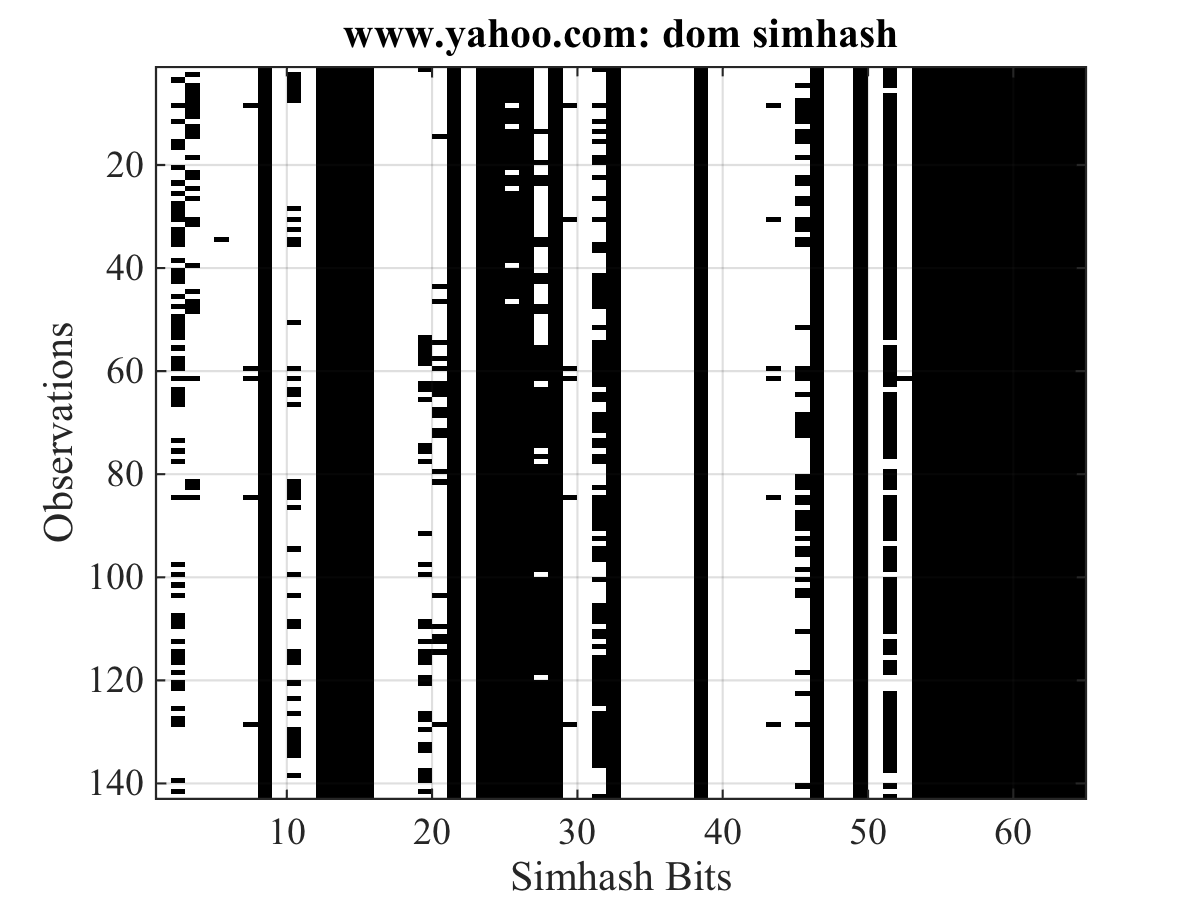
\includegraphics[width=.5\textwidth]{fig/yahoo-dom-user}
    \label{fig:yahoo-dom-user}
  \end{subfigure}%
  \begin{subfigure}
    \centering
    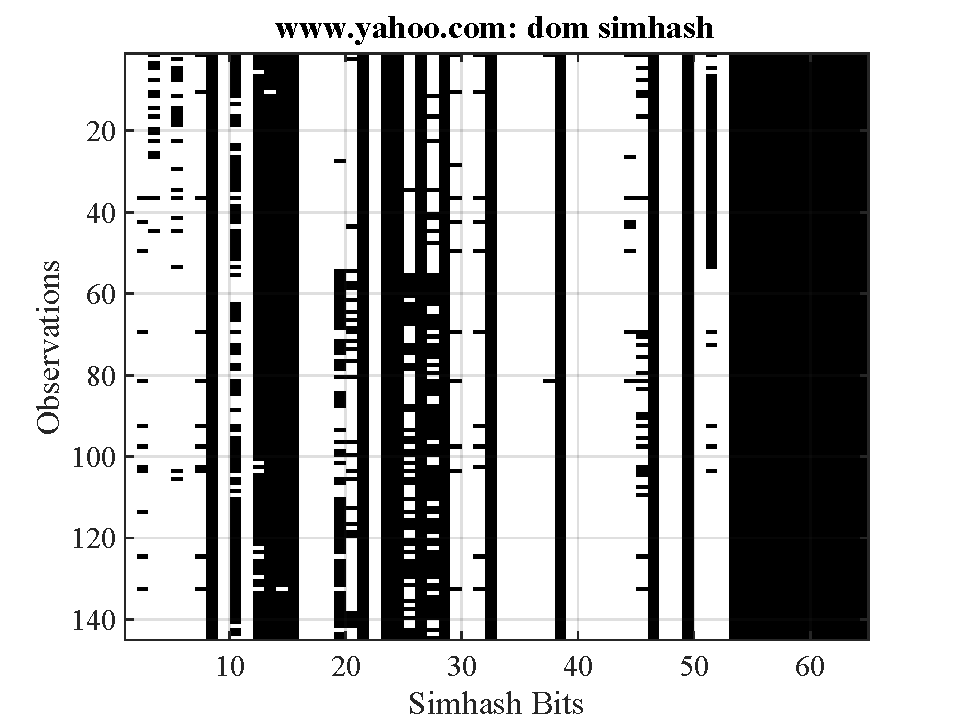
\includegraphics[width=.5\textwidth]{fig/yahoo-dom-google}
    \label{fig:yahoo-dom-google}
  \end{subfigure}
  \caption{Comparison of user and google seen dom simhash}
  \label{fig:yahoo-simhash}
\end{figure}



%In order to decide the number of clusters to take in hierarchical clustering
%(when to stop), we use inconsistent coefficient.
%
%considerations of significance, we ask whether this is an unusual result or
%whether it could have arisen merely by chance
%
%One way to determine the natural cluster divisions in a data set is to 
%linkage metric: hammming
%method: Unweighted average distance (UPGMA)
%cutoff: inconsistent value less than c
%pick inconsistent value now!!!!!
%


%\begin{gather*} \label{npa}
%  d(u,v) = \min(dist(u[i],v[j])) \\
%  \text{for all points i in cluster u and j in
%  cluster v. }
%\end{gather*}
%This~\autoref{npa} is known as the Nearest Point Algorithm.
%
%Single-linkage clustering is one of several methods of agglomerative
%hierarchical clustering. In the beginning of the process, each element is in a
%cluster of its own. The clusters are then sequentially combined into larger
%clusters, until all elements end up being in the same cluster. The stop
%criterion is the distance one.

\subsection{Cloaking Detection}
In the above section, for each website, we have learned clusters, which is
Simhash-based Website Model. In order to use SWM, let's first look at how the
comparison is going to be done. In order to detect SEO and SEM cloaking,
this work first search and click results with normal user agent, then visit 
landing urls collected with google bot user agent.
For a specific website, we denote the spider copies as $S_{spider} = s_{i}, i \in
(1,n)$, n is the number observations collected by spiders.
Denote the user observation as $s_{j}$. In order to
compare $s_{j}$ with $S_{spider}$, $S_{spider}$ is first lerned through
hierarchical clustering, and this results in $C_{spider, i}, i \in (1,c)$, c is
the number of clusters learned.

For each cluster $C_{spider, i}$, we have link heights and centroid recorded.
When comparing $s_{j}$ with $C_{spider, i}$, distance from $s_{j}$ to centroid
of $C_{spider, i}$, i.e. $d_{j,i}$ can be computed.
In order to reject $s_{j}$, we use inconsistent coefficient as well. If
\begin{equation}
  \label{coefficient:detect}
  \frac{d_{j,i} - \mu}{\sigma} > T_{detect}
\end{equation}

we reject this observation.
An observation is marked as cloaking only when all the clusters reject it.

However, in reality, there can be consistent differences between what spider
sees and what user sees and this is totally leagal. An example is, a website may
present advertisements to normal user, but non-advertisement version to spider.
Besides, there are websites that rarely changes at all. Therefore, $\sigma$ is
zero, thus ~\autoref{coefficient:detect} doesn't work. To fix the two problem, we introduce
a minimum radius $R_{detect}$. The modified formula is like this:
\begin{equation}
  \label{radius:detect}
  \frac{d_{j,i} - R_{detect} - \mu}{\sigma} > T_{detect}
\end{equation}

%Classification hinges on having access to a robust set of features derived from
%URLs to discern between spam and non-spam. Previous work has shown that lexical
%properties of URLs, page content, and hosting properties of domains are all
%effective routes for classification [15], [16], [22]–[24]. We expand upon these
%ideas, adding our own sources of features collected by one of three components:
%a web browser, a DNS resolver, and IP address analysis. A comprehensive list of
%features and the component that collects them can be found in Table 1. A single
%monitor oversees multiple copies of each component to aggregate results and
%restart failed processes. In turn, the monitor and feature collection components
%are bundled into a crawling instance and replicated in the cloud


%\subsection{Model Selection}
%
%
%\begin{table*}[!th]                                                     
%  \centering                                                            
%  \scriptsize                                                           
%  \begin{tabular}{lllllllllll}
  \toprule
  & \multicolumn{2}{c}{\textbf{Normal}}
  & \multicolumn{2}{c}{\textbf{Lognormal}}
  & \multicolumn{2}{c}{\textbf{Exponential}}
  & \multicolumn{2}{c}{\textbf{Gamma}}
  & \multicolumn{2}{c}{\textbf{Logistic}}\\

  \textbf{Website(Hash Type)\textbackslash Model}
  & AD-value
  & P-value
  & AD-value
  & P-value
  & AD-value
  & P-value
  & AD-value
  & P-value
  & AD-value
  & P-value \\
  \midrule
  digg.com T & 0.617 &  0.100 & 0.481 &  0.219 &
  14.851 & < 0.003 & 0.538 &  0.186 & 0.531 &  0.131\\ 
  digg.com T & 0.227 &  0.806 & 0.179 &  0.914 &
  19.690 &  < 0.003 & 0.198 &  > 0.250 & 0.250 & >0.250\\
  yahoo.com T & 0.192 &  0.893 & 0.263 &  0.692 &
  35.828 & <0.003 &   0.231 & >0.250 & 0.222 & >0.250\\
  amazon.com T & 0.720 &  0.058 & 0.323 &  0.520 & 
  27.754 & <0.003 &  0.436 & >0.250 & 0.642 &  0.058\\
  reddit.com T & 0.373 &  0.411 & 0.331  & 0.509 & 
  35.063 & <0.003 & 0.340 & >0.250 & 0.361 & >0.250\\
  yacombinator.com T & 0.473 &  0.237 & 0.516 &  0.186 &
  37.551 & <0.003 & 0.519 &  0.204 & 0.583 &  0.089\\

  digg.com D & 0.319 &  0.372 & 0.348 &  0.305 &
  1.491 &  0.021 &  0.402 & >0.250 & 0.363 & >0.250\\
  yahoo.com D & 0.531 &  0.168 & 0.392 &  0.366 &
  18.837 & <0.003 & 0.441 & >0.250 & 0.584  & 0.088\\
  amazon.com D & 1.519 & <0.005 & 0.916 &  0.019 &
  22.083 & <0.003 & 1.052 &  0.009 & 0.548 &  0.114\\
  amazon.com D & 0.483 & 0.117 &  0.504 & 0.104 &
  1.741 & 0.010 & 0.601 & 0.128 & 0.523 & 0.115\\

\end{tabular}

                                     
%  \caption{Model statistics for selected websites}
%  \label{tbl:para-select}                                         
%\end{table*}                                                            
%
%
%This table ~\autoref{tbl:para-select} shows the Anderson-Darling (AD) value and P-value for each model.
%A common rule used in model selection is pick the model which has the smallest
%value with P-value greater than 5\%. Each row in the table represents one
%website. From the statistics of these websites, we choose normal distribution
%for text simhash and Lognomal distribution for dom simhash.
%
%In the simhash based cloaking detection model, input from the user is simply simhash. How to compare against the simhashs that is already collected?
%
%One simple way is to compute the average distance from this simhash to all the observed simhashs. The next step is then to tell whether this distance is reasonable. 
%
%The text distribution follows lognormal distribution.
%After mannual check of those results.
%
%
%
%
%You have to run {\tt latex} once to prepare your references for
%munging.  Then run {\tt bibtex} to build your bibliography metadata.
%Then run {\tt latex} twice to ensure all references have been resolved.
%If your source file is called {\tt usenixTemplate.tex} and your {\tt
%bibtex} file is called {\tt usenixTemplate.bib}, here's what you do:
%{\tt \small
%  \begin{verbatim}
%  latex usenixTemplate
%  bibtex usenixTemplate
%  latex usenixTemplate
%  latex usenixTemplate
%  \end{verbatim}
%}
%

